\documentclass[11pt]{article}
\usepackage[margin=0.6in]{geometry}
\usepackage{amsmath, amssymb}
\usepackage{tikz}
\setlength{\parindent}{0pt}

\title{MATH 304 Exam II -- Full Step-by-Step Solutions}
\date{}

\begin{document}
\maketitle

\section*{Core Idea (Read First)}
Almost every problem reduces to one of these:
\begin{itemize}
    \item Row reduction
    \item Solving $Ax=0$
    \item Identifying pivot columns
    \item Dot product / projection formulas
\end{itemize}

\hrulefill

\section*{Problem 1: Linear Independence in $R^{2\times2}$}

We are given 4 matrices. Treat each matrix as a vector in $\mathbb{R}^4$:

\[
\begin{bmatrix} a & b \\ c & d \end{bmatrix}
\rightarrow
\begin{bmatrix} a \\ b \\ c \\ d \end{bmatrix}
\]

So we form:

\[
v_1 =
\begin{bmatrix}1\\1\\0\\-1\end{bmatrix},\quad
v_2 =
\begin{bmatrix}2\\1\\0\\-2\end{bmatrix},\quad
v_3 =
\begin{bmatrix}0\\1\\2\\0\end{bmatrix},\quad
v_4 =
\begin{bmatrix}0\\0\\1\\0\end{bmatrix}
\]

Put into matrix:

\[
A =
\begin{bmatrix}
1 & 2 & 0 & 0 \\
1 & 1 & 1 & 0 \\
0 & 0 & 2 & 1 \\
-1 & -2 & 0 & 0
\end{bmatrix}
\]

\subsection*{Row Reduction (SHOW EVERYTHING)}

Start:

\[
R_2 \leftarrow R_2 - R_1
\]

\[
\begin{bmatrix}
1 & 2 & 0 & 0 \\
0 & -1 & 1 & 0 \\
0 & 0 & 2 & 1 \\
-1 & -2 & 0 & 0
\end{bmatrix}
\]

\[
R_4 \leftarrow R_4 + R_1
\]

\[
\begin{bmatrix}
1 & 2 & 0 & 0 \\
0 & -1 & 1 & 0 \\
0 & 0 & 2 & 1 \\
0 & 0 & 0 & 0
\end{bmatrix}
\]

We now clearly have a zero row $\Rightarrow$ rank $< 4$

\subsection*{Conclusion}

\begin{itemize}
    \item Not linearly independent
    \item Do NOT span $\mathbb{R}^{2\times2}$
    \item Not a basis
\end{itemize}

\textbf{Exam Insight:}
4 vectors in $\mathbb{R}^4$ must have 4 pivots to be independent.

\hrulefill

\section*{Problem 2: Null, Row, Column Spaces}

\[
A =
\begin{bmatrix}
3 & 2 & 1 \\
10 & 8 & 6 \\
1 & 2 & 3
\end{bmatrix}
\]

\subsection*{Step 1: Row Reduce}

Swap $R_1$ and $R_3$:

\[
\begin{bmatrix}
1 & 2 & 3 \\
10 & 8 & 6 \\
3 & 2 & 1
\end{bmatrix}
\]

Eliminate below pivot:

\[
R_2 \leftarrow R_2 - 10R_1,\quad
R_3 \leftarrow R_3 - 3R_1
\]

\[
\begin{bmatrix}
1 & 2 & 3 \\
0 & -12 & -24 \\
0 & -4 & -8
\end{bmatrix}
\]

Divide $R_2$ by $-12$:

\[
\begin{bmatrix}
1 & 2 & 3 \\
0 & 1 & 2 \\
0 & -4 & -8
\end{bmatrix}
\]

Eliminate:

\[
R_3 \leftarrow R_3 + 4R_2
\]

\[
\begin{bmatrix}
1 & 2 & 3 \\
0 & 1 & 2 \\
0 & 0 & 0
\end{bmatrix}
\]

Back substitute:

\[
R_1 \leftarrow R_1 - 2R_2
\]

\[
\begin{bmatrix}
1 & 0 & -1 \\
0 & 1 & 2 \\
0 & 0 & 0
\end{bmatrix}
\]

\subsection*{(a) Null Space}

Solve:

\[
x_1 - x_3 = 0,\quad x_2 + 2x_3 = 0
\]

Let $x_3 = t$

\[
x_1 = t,\quad x_2 = -2t
\]

\[
x =
t
\begin{bmatrix}
1\\-2\\1
\end{bmatrix}
\]

\textbf{Basis:}
\[
\left\{
\begin{bmatrix}
1\\-2\\1
\end{bmatrix}
\right\}
\]

\subsection*{(b) Row Space}

Take nonzero rows:

\[
(1,0,-1), (0,1,2)
\]

\subsection*{(c) Column Space}

Pivot columns = columns 1 and 2 of ORIGINAL matrix:

\[
\left\{
\begin{bmatrix}3\\10\\1\end{bmatrix},
\begin{bmatrix}2\\8\\2\end{bmatrix}
\right\}
\]


\section*{Problem 3: Extend to a Basis of $\mathbb{R}^4$}

We are given:
\[
v_1 = (1,2,3,4)^T,\quad v_2 = (2,4,6,5)^T
\]

\subsection*{Step 1: Check if vectors are independent}

Set up:
\[
c_1 v_1 + c_2 v_2 = 0
\]

\[
c_1
\begin{bmatrix}
1\\2\\3\\4
\end{bmatrix}
+
c_2
\begin{bmatrix}
2\\4\\6\\5
\end{bmatrix}
=
\begin{bmatrix}
0\\0\\0\\0
\end{bmatrix}
\]

This gives system:
\[
\begin{cases}
c_1 + 2c_2 = 0 \\
2c_1 + 4c_2 = 0 \\
3c_1 + 6c_2 = 0 \\
4c_1 + 5c_2 = 0
\end{cases}
\]

First three equations are multiples → redundant.

Use first:
\[
c_1 = -2c_2
\]

Plug into last:
\[
4(-2c_2) + 5c_2 = -8c_2 + 5c_2 = -3c_2 = 0
\Rightarrow c_2 = 0
\Rightarrow c_1 = 0
\]

\textbf{Conclusion:} vectors are linearly independent.

\subsection*{Step 2: Extend to basis}

We need 4 independent vectors total.

Add standard basis vectors:
\[
e_1 = (1,0,0,0),\quad e_2 = (0,1,0,0)
\]

Now check if:
\[
\{v_1, v_2, e_1, e_2\}
\]
is independent.

\subsection*{Step 3: Row reduce}

Form matrix:

\[
\begin{bmatrix}
1 & 2 & 1 & 0 \\
2 & 4 & 0 & 1 \\
3 & 6 & 0 & 0 \\
4 & 5 & 0 & 0
\end{bmatrix}
\]

Row reduce:

\[
R_2 \leftarrow R_2 - 2R_1,\quad
R_3 \leftarrow R_3 - 3R_1,\quad
R_4 \leftarrow R_4 - 4R_1
\]

\[
\begin{bmatrix}
1 & 2 & 1 & 0 \\
0 & 0 & -2 & 1 \\
0 & 0 & -3 & 0 \\
0 & -3 & -4 & 0
\end{bmatrix}
\]

Swap $R_2$ and $R_4$:

\[
\begin{bmatrix}
1 & 2 & 1 & 0 \\
0 & -3 & -4 & 0 \\
0 & 0 & -3 & 0 \\
0 & 0 & -2 & 1
\end{bmatrix}
\]

Continue → 4 pivots exist → independent.

\subsection*{Final Answer}

A valid basis:
\[
\left\{
(1,2,3,4),\,
(2,4,6,5),\,
(1,0,0,0),\,
(0,1,0,0)
\right\}
\]

\textbf{Exam Insight:}
\begin{itemize}
    \item Start with given independent set
    \item Add standard basis vectors
    \item Only row reduce if unsure
\end{itemize}

\hrulefill

\section*{Problem 4: Find a Basis for $\mathbb{R}^3$}

Given set:
\[
\{(1,2,3), (2,0,1), (4,-4,-3), (1,1,1), (0,-6,-6)\}
\]

\subsection*{Step 1: Put vectors as columns}

\[
A =
\begin{bmatrix}
1 & 2 & 4 & 1 & 0 \\
2 & 0 & -4 & 1 & -6 \\
3 & 1 & -3 & 1 & -6
\end{bmatrix}
\]

\subsection*{Step 2: Row reduce}

Start:

\[
R_2 \leftarrow R_2 - 2R_1,\quad
R_3 \leftarrow R_3 - 3R_1
\]

\[
\begin{bmatrix}
1 & 2 & 4 & 1 & 0 \\
0 & -4 & -12 & -1 & -6 \\
0 & -5 & -15 & -2 & -6
\end{bmatrix}
\]

Eliminate:

\[
R_3 \leftarrow R_3 - \frac{5}{4}R_2
\]

\[
\begin{bmatrix}
1 & 2 & 4 & 1 & 0 \\
0 & -4 & -12 & -1 & -6 \\
0 & 0 & 0 & -\frac{3}{4} & \frac{3}{2}
\end{bmatrix}
\]

Now scale:

\[
R_2 \leftarrow -\frac{1}{4}R_2
\]

\[
\begin{bmatrix}
1 & 2 & 4 & 1 & 0 \\
0 & 1 & 3 & \frac{1}{4} & \frac{3}{2} \\
0 & 0 & 0 & -\frac{3}{4} & \frac{3}{2}
\end{bmatrix}
\]

Make pivot in row 3:

\[
R_3 \leftarrow -\frac{4}{3}R_3
\]

\[
\begin{bmatrix}
1 & 2 & 4 & 1 & 0 \\
0 & 1 & 3 & \frac{1}{4} & \frac{3}{2} \\
0 & 0 & 0 & 1 & -2
\end{bmatrix}
\]

\subsection*{Step 3: Identify pivot columns}

Pivot columns: 1, 2, 4

\subsection*{Final Answer}

Basis:
\[
\left\{
(1,2,3),\,
(2,0,1),\,
(1,1,1)
\right\}
\]

\textbf{Exam Insight:}
\begin{itemize}
    \item Always take pivot columns from ORIGINAL vectors
    \item You only need 3 vectors in $\mathbb{R}^3$
\end{itemize}

\hrulefill

\section*{Problem 5: Coordinate Vector Relative to a Basis}

We are given a basis:
\[
S =
\left\{
\begin{bmatrix}1 & 0 \\ 0 & 0\end{bmatrix},
\begin{bmatrix}1 & 0 \\ 0 & 2\end{bmatrix},
\begin{bmatrix}1 & 2 \\ 0 & 3\end{bmatrix},
\begin{bmatrix}1 & 1 \\ 1 & 1\end{bmatrix}
\right\}
\]

We want the coordinate vector of:
\[
A =
\begin{bmatrix}
-1 & 1 \\
-3 & 1
\end{bmatrix}
\]

\subsection*{Step 1: Set up linear combination}

We are solving:
\[
c_1 S_1 + c_2 S_2 + c_3 S_3 + c_4 S_4 = A
\]

Write explicitly:

\[
c_1
\begin{bmatrix}1 & 0 \\ 0 & 0\end{bmatrix}
+
c_2
\begin{bmatrix}1 & 0 \\ 0 & 2\end{bmatrix}
+
c_3
\begin{bmatrix}1 & 2 \\ 0 & 3\end{bmatrix}
+
c_4
\begin{bmatrix}1 & 1 \\ 1 & 1\end{bmatrix}
=
\begin{bmatrix}-1 & 1 \\ -3 & 1\end{bmatrix}
\]

\subsection*{Step 2: Add matrices component-wise}

Top-left entry:
\[
c_1 + c_2 + c_3 + c_4 = -1
\]

Top-right entry:
\[
2c_3 + c_4 = 1
\]

Bottom-left entry:
\[
c_4 = -3
\]

Bottom-right entry:
\[
2c_2 + 3c_3 + c_4 = 1
\]

\subsection*{Step 3: Solve system}

From bottom-left:
\[
c_4 = -3
\]

Plug into second equation:
\[
2c_3 - 3 = 1 \Rightarrow 2c_3 = 4 \Rightarrow c_3 = 2
\]

Plug into fourth:
\[
2c_2 + 3(2) - 3 = 1
\]

\[
2c_2 + 6 - 3 = 1
\Rightarrow 2c_2 + 3 = 1
\Rightarrow 2c_2 = -2
\Rightarrow c_2 = -1
\]

Now use first equation:
\[
c_1 + (-1) + 2 + (-3) = -1
\]

\[
c_1 -2 = -1
\Rightarrow c_1 = 1
\]

\subsection*{Final Answer}

\[
[A]_S =
\begin{bmatrix}
1 \\ -1 \\ 2 \\ -3
\end{bmatrix}
\]

\subsection*{Interpretation (IMPORTANT)}

This means:
\[
A = 1S_1 - 1S_2 + 2S_3 - 3S_4
\]

\textbf{Exam Insight:}
\begin{itemize}
    \item This is just solving $[S]c = A$
    \item Treat matrices as vectors in $\mathbb{R}^4$
    \item Match entries position-by-position
\end{itemize}

\hrulefill

\section*{Problem 6: Linear Transformations and Change of Basis}

We are given:
\[
f : \mathbb{R}^3 \to \mathbb{R}^2,\quad
f(x) =
\begin{bmatrix}
x_1 - x_2 \\
x_2 + 2x_3
\end{bmatrix}
\]

\subsection*{(a) Find the standard matrix of $f$}

\textbf{Key idea:}
The standard matrix is:
\[
A = [f(e_1)\; f(e_2)\; f(e_3)]
\]

where:
\[
e_1 = (1,0,0),\quad e_2 = (0,1,0),\quad e_3 = (0,0,1)
\]

\subsection*{Step 1: Compute $f(e_1)$}

\[
f(1,0,0) =
\begin{bmatrix}
1 - 0 \\
0 + 2(0)
\end{bmatrix}
=
\begin{bmatrix}
1 \\
0
\end{bmatrix}
\]

\subsection*{Step 2: Compute $f(e_2)$}

\[
f(0,1,0) =
\begin{bmatrix}
0 - 1 \\
1 + 0
\end{bmatrix}
=
\begin{bmatrix}
-1 \\
1
\end{bmatrix}
\]

\subsection*{Step 3: Compute $f(e_3)$}

\[
f(0,0,1) =
\begin{bmatrix}
0 - 0 \\
0 + 2
\end{bmatrix}
=
\begin{bmatrix}
0 \\
2
\end{bmatrix}
\]

\subsection*{Step 4: Form matrix}

\[
A =
\begin{bmatrix}
1 & -1 & 0 \\
0 & 1 & 2
\end{bmatrix}
\]

\textbf{Answer (a):}
\[
A =
\begin{bmatrix}
1 & -1 & 0 \\
0 & 1 & 2
\end{bmatrix}
\]

\hrulefill

\subsection*{(b) Matrix relative to new bases}

We are given:

Domain basis:
\[
v_1 = (1,0,1),\;
v_2 = (1,1,0),\;
v_3 = (0,1,1)
\]

Codomain basis:
\[
u_1 = (1,1),\quad u_2 = (1,-1)
\]

\textbf{Goal:}
Find $[f]_{U,V}$

\subsection*{BIG IDEA (this is the test concept)}

We compute:
\[
[f]_{U,V} = P_U^{-1} \; A \; P_V
\]

where:
\begin{itemize}
    \item $P_V$ = matrix with $v_i$ as columns
    \item $P_U$ = matrix with $u_i$ as columns
\end{itemize}

\hrulefill

\subsection*{Step 1: Build $P_V$}

\[
P_V =
\begin{bmatrix}
1 & 1 & 0 \\
0 & 1 & 1 \\
1 & 0 & 1
\end{bmatrix}
\]

\subsection*{Step 2: Build $P_U$}

\[
P_U =
\begin{bmatrix}
1 & 1 \\
1 & -1
\end{bmatrix}
\]

\subsection*{Step 3: Compute $P_U^{-1}$}

Determinant:
\[
\det(P_U) = (1)(-1) - (1)(1) = -2
\]

\[
P_U^{-1}
=
\frac{1}{-2}
\begin{bmatrix}
-1 & -1 \\
-1 & 1
\end{bmatrix}
=
\begin{bmatrix}
\frac{1}{2} & \frac{1}{2} \\
\frac{1}{2} & -\frac{1}{2}
\end{bmatrix}
\]

\hrulefill

\subsection*{Step 4: Compute $A P_V$}

\[
A =
\begin{bmatrix}
1 & -1 & 0 \\
0 & 1 & 2
\end{bmatrix}
\quad
P_V =
\begin{bmatrix}
1 & 1 & 0 \\
0 & 1 & 1 \\
1 & 0 & 1
\end{bmatrix}
\]

Multiply column-by-column:

\textbf{First column:}
\[
A v_1 =
\begin{bmatrix}
1 & -1 & 0 \\
0 & 1 & 2
\end{bmatrix}
\begin{bmatrix}
1 \\ 0 \\ 1
\end{bmatrix}
=
\begin{bmatrix}
1 \\
2
\end{bmatrix}
\]

\textbf{Second column:}
\[
A v_2 =
\begin{bmatrix}
1 \\ 1
\end{bmatrix}
\]

\textbf{Third column:}
\[
A v_3 =
\begin{bmatrix}
-1 \\
3
\end{bmatrix}
\]

So:
\[
A P_V =
\begin{bmatrix}
1 & 1 & -1 \\
2 & 1 & 3
\end{bmatrix}
\]

\hrulefill

\subsection*{Step 5: Multiply $P_U^{-1}(A P_V)$}

\[
P_U^{-1} =
\begin{bmatrix}
\frac{1}{2} & \frac{1}{2} \\
\frac{1}{2} & -\frac{1}{2}
\end{bmatrix}
\]

Multiply each column:

\textbf{Column 1:}
\[
\begin{bmatrix}
\frac{1}{2}(1) + \frac{1}{2}(2) \\
\frac{1}{2}(1) - \frac{1}{2}(2)
\end{bmatrix}
=
\begin{bmatrix}
\frac{3}{2} \\
-\frac{1}{2}
\end{bmatrix}
\]

\textbf{Column 2:}
\[
\begin{bmatrix}
1 \\
0
\end{bmatrix}
\]

\textbf{Column 3:}
\[
\begin{bmatrix}
1 \\
-2
\end{bmatrix}
\]

\subsection*{Final Answer}

\[
[f]_{U,V} =
\begin{bmatrix}
\frac{3}{2} & 1 & 1 \\
-\frac{1}{2} & 0 & -2
\end{bmatrix}
\]

\hrulefill

\subsection*{Interpretation (VERY IMPORTANT)}

\begin{itemize}
    \item $P_V$: converts from $V$-coordinates to standard
    \item $A$: applies transformation
    \item $P_U^{-1}$: converts result into $U$-coordinates
\end{itemize}

So:
\[
\text{new coords} = (\text{change output}) \circ f \circ (\text{change input})
\]

\textbf{Exam Insight:}
If you forget formula, think:
\begin{center}
\textit{“Go to standard → apply $A$ → go to new basis”}
\end{center}

\hrulefill

\section*{Problem 7: Geometry in $\mathbb{R}^3$}

We are given:
\[
x = (1,2,3), \quad v = (3,2,1)
\]

\subsection*{Step 1: Compute the dot product}

\[
x \cdot v = (1)(3) + (2)(2) + (3)(1)
\]

\[
= 3 + 4 + 3 = 10
\]

\hrulefill

\subsection*{Step 2: Compute magnitudes}

\[
||x|| = \sqrt{1^2 + 2^2 + 3^2}
= \sqrt{1 + 4 + 9}
= \sqrt{14}
\]

\[
||v|| = \sqrt{3^2 + 2^2 + 1^2}
= \sqrt{9 + 4 + 1}
= \sqrt{14}
\]

\hrulefill

\subsection*{(a) Distance between $x$ and $v$}

Distance = magnitude of difference:

\[
x - v = (1-3,\; 2-2,\; 3-1)
= (-2, 0, 2)
\]

\[
||x - v|| =
\sqrt{(-2)^2 + 0^2 + 2^2}
= \sqrt{4 + 0 + 4}
= \sqrt{8}
\]

\[
= 2\sqrt{2}
\]

\textbf{Answer:} $2\sqrt{2}$

\hrulefill

\subsection*{(b) Angle between $x$ and $v$}

Formula:
\[
\cos\theta =
\frac{x \cdot v}{||x||\,||v||}
\]

\[
\cos\theta =
\frac{10}{\sqrt{14}\cdot \sqrt{14}}
=
\frac{10}{14}
=
\frac{5}{7}
\]

\[
\theta = \cos^{-1}\left(\frac{5}{7}\right)
\]

\textbf{Answer:}
\[
\theta = \cos^{-1}(5/7)
\]

\textbf{Interpretation:}
Vectors are somewhat aligned (since cosine is positive and fairly large).

\hrulefill

\subsection*{(c) Scalar projection of $x$ onto $v$}

Formula:
\[
\text{comp}_v x =
\frac{x \cdot v}{||v||}
\]

\[
=
\frac{10}{\sqrt{14}}
\]

\textbf{Answer:}
\[
\frac{10}{\sqrt{14}}
\]

\textbf{Meaning:}
This is the signed length of the ``shadow'' of $x$ onto $v$.

\hrulefill

\subsection*{(d) Vector projection of $x$ onto $v$}

Formula:
\[
\text{proj}_v x =
\frac{x \cdot v}{||v||^2} v
\]

\[
=
\frac{10}{14} v
=
\frac{5}{7}(3,2,1)
\]

\[
=
\left(
\frac{15}{7}, \frac{10}{7}, \frac{5}{7}
\right)
\]

\textbf{Answer:}
\[
\left(
\frac{15}{7}, \frac{10}{7}, \frac{5}{7}
\right)
\]

\hrulefill

\subsection*{Geometric Visualization}

\begin{center}
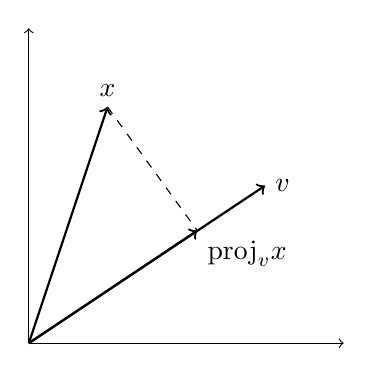
\begin{tikzpicture}[scale=1]

% axes
\draw[->] (0,0) -- (4,0);
\draw[->] (0,0) -- (0,4);

% vectors
\draw[->, thick] (0,0) -- (3,2) node[right] {$v$};
\draw[->, thick] (0,0) -- (1,3) node[above] {$x$};

% projection
\draw[dashed] (1,3) -- (2.14,1.43);
\draw[->, thick] (0,0) -- (2.14,1.43) node[below right] {$\text{proj}_v x$};

\end{tikzpicture}
\end{center}

\textbf{Key intuition:}
\begin{itemize}
    \item Projection = ``shadow'' of $x$ onto $v$
    \item Scalar projection = length of that shadow
    \item Vector projection = actual vector along $v$
\end{itemize}

\hrulefill

\subsection*{Exam Pattern Recognition}

\begin{itemize}
    \item Dot product shows up everywhere
    \item Angle = dot product formula
    \item Projection = SAME dot product reused
    \item Distance = just a norm
\end{itemize}

\hrulefill

\section*{Problem 8: Closest Point to a Plane}

We are given the plane:
\[
2(x - 1) + 3(y + 1) - z = 0
\]

We want the point on the plane closest to the origin $(0,0,0)$.

\hrulefill

\subsection*{Step 1: Rewrite plane in standard form}

Expand:
\[
2x - 2 + 3y + 3 - z = 0
\]

\[
2x + 3y - z + 1 = 0
\]

So plane is:
\[
2x + 3y - z = -1
\]

\hrulefill

\subsection*{Step 2: Identify the normal vector}

The normal vector comes from coefficients:
\[
\mathbf{n} = (2,3,-1)
\]

\textbf{Key idea:}
The closest point from the origin to the plane lies \textbf{along the normal direction}.

\hrulefill

\subsection*{Step 3: Parametrize the line from origin along the normal}

Any point on this line:
\[
\mathbf{p}(t) = t(2,3,-1)
\]

\[
= (2t, 3t, -t)
\]

\hrulefill

\subsection*{Step 4: Plug into plane equation}

Substitute into:
\[
2x + 3y - z = -1
\]

\[
2(2t) + 3(3t) - (-t) = -1
\]

\[
4t + 9t + t = -1
\]

\[
14t = -1
\Rightarrow t = -\frac{1}{14}
\]

\hrulefill

\subsection*{Step 5: Find the point}

\[
\mathbf{p} =
\left(
2\left(-\frac{1}{14}\right),
3\left(-\frac{1}{14}\right),
-\left(-\frac{1}{14}\right)
\right)
\]

\[
=
\left(
-\frac{2}{14},\;
-\frac{3}{14},\;
\frac{1}{14}
\right)
\]

Simplify:
\[
=
\left(
-\frac{1}{7},\;
-\frac{3}{14},\;
\frac{1}{14}
\right)
\]

\subsection*{Final Answer}

\[
\boxed{
\left(
-\frac{1}{7},\;
-\frac{3}{14},\;
\frac{1}{14}
\right)
}
\]

\hrulefill

\subsection*{Geometric Visualization}

\begin{center}
\begin{tikzpicture}[scale=1]

% axes
\draw[->] (0,0) -- (4,0);
\draw[->] (0,0) -- (0,4);

% plane line (2D representation)
\draw[thick] (-1,3) -- (3,-1) node[right] {plane};

% origin
\fill (0,0) circle (2pt) node[below left] {0};

% projection point
\fill (0.6,0.4) circle (2pt);

% normal direction
\draw[->, thick] (0,0) -- (1.2,0.8) node[right] {$\mathbf{n}$};

% perpendicular drop
\draw[dashed] (0,0) -- (0.6,0.4);

\end{tikzpicture}
\end{center}

\textbf{Key intuition:}
\begin{itemize}
    \item Shortest distance = perpendicular distance
    \item Perpendicular direction = normal vector
    \item So we move along $\mathbf{n}$ until we hit the plane
\end{itemize}

\hrulefill

\subsection*{Exam Pattern Recognition}

If you see:
\begin{itemize}
    \item ``closest point to plane''
    \item ``distance to plane''
\end{itemize}

\textbf{Immediately think:}
\begin{center}
\textit{normal vector + projection}
\end{center}

\hrulefill

\section*{Problem 9: Orthogonal Complement}

We are given:
\[
v_1 =
\begin{bmatrix}
1\\1\\2\\3
\end{bmatrix},
\quad
v_2 =
\begin{bmatrix}
0\\3\\2\\1
\end{bmatrix}
\]

We want a basis for:
\[
\text{Span}(v_1, v_2)^\perp
\]

\hrulefill

\subsection*{Step 1: Translate definition}

A vector $x = (x_1,x_2,x_3,x_4)$ is in the orthogonal complement if:
\[
x \cdot v_1 = 0 \quad \text{and} \quad x \cdot v_2 = 0
\]

\hrulefill

\subsection*{Step 2: Write equations}

Dot with $v_1$:
\[
x_1 + x_2 + 2x_3 + 3x_4 = 0
\]

Dot with $v_2$:
\[
0x_1 + 3x_2 + 2x_3 + x_4 = 0
\]

So system:
\[
\begin{cases}
x_1 + x_2 + 2x_3 + 3x_4 = 0 \\
3x_2 + 2x_3 + x_4 = 0
\end{cases}
\]

\hrulefill

\subsection*{Step 3: Solve system}

Solve second equation for $x_2$:
\[
3x_2 = -2x_3 - x_4
\Rightarrow
x_2 = -\frac{2}{3}x_3 - \frac{1}{3}x_4
\]

Plug into first equation:

\[
x_1 + \left(-\frac{2}{3}x_3 - \frac{1}{3}x_4\right) + 2x_3 + 3x_4 = 0
\]

Combine like terms:

\[
x_1 + \left(2 - \frac{2}{3}\right)x_3 + \left(3 - \frac{1}{3}\right)x_4 = 0
\]

\[
x_1 + \frac{4}{3}x_3 + \frac{8}{3}x_4 = 0
\]

Solve for $x_1$:

\[
x_1 = -\frac{4}{3}x_3 - \frac{8}{3}x_4
\]

\hrulefill

\subsection*{Step 4: Parametrize solution}

Let:
\[
x_3 = s,\quad x_4 = t
\]

Then:
\[
x_2 = -\frac{2}{3}s - \frac{1}{3}t
\]

\[
x_1 = -\frac{4}{3}s - \frac{8}{3}t
\]

So:
\[
x =
\begin{bmatrix}
-\frac{4}{3}s - \frac{8}{3}t \\
-\frac{2}{3}s - \frac{1}{3}t \\
s \\
t
\end{bmatrix}
\]

\hrulefill

\subsection*{Step 5: Write as linear combination}

\[
x =
s
\begin{bmatrix}
-\frac{4}{3} \\
-\frac{2}{3} \\
1 \\
0
\end{bmatrix}
+
t
\begin{bmatrix}
-\frac{8}{3} \\
-\frac{1}{3} \\
0 \\
1
\end{bmatrix}
\]

To clean up (remove fractions), multiply each vector:

First vector $\times 3$:
\[
\begin{bmatrix}
-4 \\ -2 \\ 3 \\ 0
\end{bmatrix}
\]

Second vector $\times 3$:
\[
\begin{bmatrix}
-8 \\ -1 \\ 0 \\ 3
\end{bmatrix}
\]

\subsection*{Final Answer}

A basis for the orthogonal complement is:
\[
\boxed{
\left\{
\begin{bmatrix}
-4 \\ -2 \\ 3 \\ 0
\end{bmatrix},
\begin{bmatrix}
-8 \\ -1 \\ 0 \\ 3
\end{bmatrix}
\right\}
}
\]

\hrulefill

\subsection*{BIG Concept Connection (VERY IMPORTANT)}

\[
\text{Span}(v_1, v_2)^\perp
=
\text{Null}(A)
\quad \text{where} \quad
A =
\begin{bmatrix}
v_1^T \\
v_2^T
\end{bmatrix}
\]

\textbf{This means:}
\begin{itemize}
    \item Orthogonal complement problems = null space problems
    \item Always turn dot products into a matrix system
\end{itemize}

\hrulefill

\subsection*{Dimension Check (Quick sanity check)}

\begin{itemize}
    \item Space is $\mathbb{R}^4$
    \item Span$(v_1,v_2)$ has dimension 2
    \item Orthogonal complement must have dimension:
\end{itemize}

\[
4 - 2 = 2
\]

We found 2 vectors $\checkmark$

\hrulefill

\subsection*{Final Exam Insight}

If you see:
\begin{itemize}
    \item ``orthogonal complement''
    \item ``perpendicular to span''
\end{itemize}

\textbf{Immediately do:}
\begin{enumerate}
    \item Write dot product equations
    \item Solve as a system
    \item Express in parametric vector form
\end{enumerate}

\hrulefill

\section*{Final Pattern Recognition}

\begin{itemize}
    \item Independence → row reduce
    \item Basis → pivots
    \item Null space → free variables
    \item Geometry → dot product
    \item Planes → normal vectors
\end{itemize}

\end{document}